\documentclass[10pt,letterpaper,onecolumn,draftclsnofoot,journal]{IEEEtran}
\usepackage[margin=0.75in]{geometry}
\usepackage{listings}
\usepackage{color}
\usepackage{longtable}
\usepackage{graphicx}
\usepackage{caption}
\usepackage{float}
\usepackage{tabu}
\usepackage{enumitem}
\usepackage{courier}
\usepackage[hidelinks]{hyperref}

\setlength{\parindent}{0cm}
\setcounter{secnumdepth}{1}

\begin{document}
\begin{titlepage}
	\title{The ARLISS Project\\Progress Report\\Senior Capstone}
	\author{Steven Silvers, Paul Minner, Zhaolong Wu, Zachary DeVita\\
		Capstone Group 27\\2016-17 Academic Year}
	\date{\today}
	\maketitle
	\vspace{4cm}
	\begin{abstract}
		\noindent This document details our experiences designing our project over the duration of the academic year. This includes progress made, problems encountered, and plans for the future. We also detail changes we plan to implement in the future.
	\end{abstract}

\end{titlepage}
\tableofcontents
\clearpage

\section{Introduction}
This document is a progress report which details our team's progress on the ARLISS Project throughout the Fall term of 2016. It  contains a week by week summary of all related activities, problems we have encountered, solutions to prior problems, and a detailed retrospective of the academic year. The retrospective will contain a section for things which have gone well, a section for changes which need to be implemented, and a section which will detail actions which will need to occur to make those changes.  

\section{Summary of Fall Term}
\subsection{Week 3}
By week 3 our team was established, we had met with our mentor and client for the first time, and our team had also met with our extended team of electrical and mechanical engineers. In class we had been briefly described upcoming assignments for our project, as well as, had been assigned the Problem Statement. Our project, the ARLISS Project, is to build a satellite, i.e. robot, and compete in the ARLISS competition. ARLISS stands for "A Rocket Launch for International Student Satellites," and it is a national competition where teams comprised of multiple engineering disciplines build a "soda-can" sized satellite which must autonomously navigate to a specified location after being ejected from a rocket at approximately 12,000' AGL and landing safely on the ground.\vspace{.3cm}
\par
The first assignment, as mentioned prior, was the Problem Statement. The problem statement is a document which was written after meeting with our team's client, and it contains a definition of the problem, for which our team is providing a software solution for, and it includes some of the specific details for our project as prescribed by the client. This document is the predecessor to the Requirements Document and is meant to serve as a "10,000 ft." view of the project with less of a focus on the specifics or how to implement the software.\vspace{.3cm}
\par 
At the end of the third week our team had not yet finished the Problem Statement. Our team initially had some difficulty meeting with our client and our extended team, i.e. the mechanical and electrical engineers. The assignment due date was pushed back a few days, but it was nearly finished at that point anyway.\vspace{.3cm}
\par 
We met with our client near the end of the third week. Her input was extraordinarily limited which has proven to be both good and bad. Our client is completely leaving all decisions regarding the project up to us. This allows us to have complete freedom for the project, and it allows us to not need to meet with her very often, but it also leaves us with no expertise or direction for the project. With all things considered, I think this may result in more of a hindrance than a benefit.

\subsection{Week 4}
The beginning of week four was spent finishing up the rough draft of the Problem Statement, getting it signed by our client, and turning it in. We managed to finish the rough draft by our extended due date without any additional issues. The team seems to work well together; everyone does their part, we are able to keep in excellent communication, and everyone seems more than capable of meeting their deadlines.\vspace{.3cm}
\par 
In addition to turning in the final draft of the Problem Statement, we also met had a meeting with our mentor on Monday of the week. We were able to speak with him about changes that would need to be made in our Problem Statement, as well as, briefly discuss some of the upcoming assignments. He was able to help clarify some of the confusion in the Problem Statement assignment description and point us in the right direction\vspace{.3cm}
\par. 
We also met with our extended team on Tuesday to discuss the project. The requirements for the competition are very open-ended so we spent most of the meeting trying to narrow down our team's specific design for the project. A requirement for the competition is that the satellite autonomously navigates to the target destination after in lands back on Earth, but there is no requirement for whether the satellite flies or drives on the ground. This is one of the major decisions made at this meeting. We decided for our satellite to autonomously drive to its destination. This was primarily due to the fact that our satellite will only weigh approximately 150 grams and even the slightest wind in the wrong direction would prevent it from reaching the target. This and the fact that a quadcopter would require much more energy to power itself, and battery power is our most critical resource for our project. We discussed the other components for the project like programming languages and design of the satellite, but nothing else was set in concrete.\vspace{.3cm}
\par   
For the remainder of the week, our team worked on incorporating some of the changes recommended by our mentor, as well as, the changes recommended by our instructors. Much of the formatting for the document was not finished in the prior week so this was a major focus for the week as well. As for plans for the following week, our team had discussed the Requirements document briefly, as a preparatory measure. The final draft of the Problem Statement would be turned in early in the next week, and the Requirements document would be the primary focus for the rest of the week. 

\subsection{Week 5}
Our team wrapped up the Problem Statement over the weekend, and we got it signed by our client on Monday morning.  The final draft of the assignment was finished and turned in on time without any issues. Again, our team met with our mentor on Monday morning, as well as, our extended team on Tuesday evening. For this week, the primary goal was to finish a rough draft of the Requirements document.\vspace{.3cm}
\par
When we met with our mentor we discussed the Requirements document. There was a bit of confusion in regards to this assignment to say the least. He was able to answer a few of the questions we had, but this only served to marginally dilute the confusion.
Our team had a considerably difficult time planning for this assignment. This document is a contract between the engineers and the client and it is intended to strictly define the tasks which our team is intended to complete. Our team, with collaboration from the extended team of engineers who are additionally working on this project, have been given full reign for the design and implementation of the project. We are solely responsible for the entire design of the project with no outside input or expertise. This means we, as a team, had to essentially develop our own requirements based on a few vague competition guidelines from their website and some educated “assumptions.”\vspace{.3cm}
\par 
Even knowing we had to develop our own requirements did not suffice. The hardware for our project had not been determined at this point and the guidelines for the competition were not available. The hardware for our project will not be available until some point in the middle of winter term. This greatly limited our team's ability to write a realistic, legitimate set of requirements. For our circumstances it seems that it would have been far more advantageous to write this document after the research had been done, but our team also understands that not all team circumstances are the same as ours.\vspace{.3cm}
\par
Either way, our team discussed the assignment in detail. We were able to brainstorm ideas for the document and delegate sections of the assignment to each of the members in our team so that we could complete the assignment. We managed to turn in a rough draft towards the end of the week. After the rough draft was turned in, the class as a whole was instructed by Dr. Kevin McGrath to spend the weekend revising our rough drafts and turning in an alternate version of the rough draft. Apparently there were enough teams equally as confused as us over the expectations of the document that it was necessary to give some clarification to the entire class and an extension on the rough draft.\vspace{.3cm}
\par 
The plan for the following week was to implement the changes which were recommended by our instructors for the rough draft of the Requirements document, and then work on the final draft of the assignment.

\subsection{Week 6}
\par
Our main accomplishment of week 6 was finishing up the requirements document. We took the document to our mentor get it signed, and talk to her about our project. She told us our plans look good so far. Once the requirements document was done, we had a better idea of what needed to be added to our software, and what technologies needed to be used. We began thinking about our next document, the technology review. In order to do this, we began researching various autonomous navigation systems to determine what we need.\vspace{.3cm}
\par
Our all-group meeting was canceled this week, so we didn't get a chance to talk to the rest of the team about different navigation systems. This wasn't a big deal, though, because we would have more time to research various systems, and talk about it at the next meeting.\vspace{.3cm}
\par
The plan for the following week was to begin writing our technology review, which means we would have to divide the project into 12 different technologies. In addition, we hoped to meet with the entire team to discuss the sensors we would have available to us for the autonomous navigation system.\vspace{.3cm}

\subsection{Week 7}
\par
This week, we finished the majority of our technology review. To do this, we had to meet and divide the project up into 12 technologies. These technologies varied from what language to implement the software in, to object recognition, to parachute deployment. Since the technologies have been researched, we could start thinking about the implementation of these technologies for the design document.\vspace{.3cm}
\par
We did not hold our all-group meeting this week, which did present a problem. That was we still didn't have a definite answer of what sensors are being used, because the ECE team is responsible for the sensors. This meant we had to make some assumptions while writing our technology review. Some of these assumptions were incorrect, and the technology review will need to be updated in the future.\vspace{.3cm}
\par
The plan for the following week was to make final edits to the technology review, and begin working on the design document. A problem that we have realized is the satellite will be designed at the same time as we are writing the software. This will make testing our software difficult. We realized we would have to start thinking about ways to test our software without the hardware it is designed to run on.\vspace{.3cm}

\subsection{Week 8}
\par
Week eight was highlighted by making final edits to and submitting our technology review for grading. Once the technology review was done and behind us we began focusing on the next assignment, the design document. Work on the design document in week eight was focused around planning out how to approach the document and the overall outline for what it will look like.\vspace{.3cm}
\par
We held our all-group meeting with the mechanical and electrical engineering sub-teams on Tuesday night where we further discussed the hardware implementation of our project. Some of the decisions made included using GPS to calculate altitude for parachute deployment, using a 9V 1200~1500 mA battery for the main power supply, as well as using two motors for driving. It is still undecided as to what kind of sensor will be used for detecting obstacles, whether it will be an image sensor or SONAR/RADAR. This raises a problem because the decision as to what kind of sensor to use directly impacts how our design document will be written and if our technology review will need revision.\vspace{.3cm}
\par
The plan for week nine is to write the design document and finish it early so we have more time to focus on the final progress report and presentation. There will be another all-group meeting where we will hopefully finalize our decision as to what kind of sensor we will be using to detect and avoid obstacles. We are still brainstorming how we would like to approach the progress report in the following weeks, whether we will record as a group or individually and then splice our presentations together.\vspace{.3cm}
\par

\subsection{Week 9}

A lot of work done during week nine was done individually as it fell on the Thanksgiving holiday break. Most of the team finished their individual portions for the design document over break, which was fairly easy to do without much collaboration as each person was responsible for writing up the same sections they wrote about in the technology review. We held our usual all-group meeting Tuesday night, where further discussion was had in regards to sensors and other design aspects of the project. It was decided that a CMOS imaging sensor would be used to detect objects in the satellite's path.\vspace{.3cm}
\par
It is still uncertain what kind of control board the electrical team will implement for the project. It currently looks like they are between using a Raspberry PI Zero and building their own custom board with an ATMega128 chip. This decision will hopefully be made soon as ultimately effects how our overall system will be designed and implemented.\vspace{.3cm}
\par
The plan for week ten is to work on the progress report early, and finish the presentation the weekend before finals week. We decided to meet as a group in a study room on campus Sunday afternoon to record the audio and screen capture for the presentation. It was decided that each person would be responsible for a portion of the progress report, and then to prepare their own speaking portions for the presentations and arrive Sunday ready to record. Steven volunteered his Engr webspace for hosting the project submission.\vspace{.3cm}

\subsection{Week 10}
During week 10, our team managed to finish the majority of our Design Document over the weekend so there was not too much time spent working on it. Everyone did there part and researched their topics, wrote up their portions of the document, and we managed to get it turned in on time. We also made sure to get a considerable head start on our progress report.\vspace{.3cm} 
\par
For the progress report, we decided to split the weeks up and each write a couple weeks. We wrote the rest of the progess report and starting to play around with the video recording tools.\vspace{.3cm}
\par
For the future hardware desgin, the electrical engineers apparently want to use an AtMega128 processor. We suspect that it is only because that is what they are accustomed to and not because it is the best tool for the job. Ideas for sensors were also mentioned. Hopefully they consider the CMOS and the ultrasonic sensors that we researched and suggested to them. During the week we also got the specifications for the competition. Our team plans on putting forth some effort and working on this project over break which would be nice. We've requested some supplies from Dr. McGrath so that hopefully we are able to work on some of the coding over the winter break.\vspace{.3cm} 
\par

\section{A Reflection of Development Period}
\begin{tabular}{ |p{0.3\linewidth}|p{0.3\linewidth}|p{0.3\linewidth}|  }
\hline
\multicolumn{3}{|c|}{Retrospective} \\
\hline
Positives& Deltas &Actions \\
\hline
Our group works well together. &
Better understand version control.&
Each group member will research Github and version control in general. \\

All software components seem possible to implement. &
Better implement version control &
Start submitting changes to Github via Pull Request instead of Pushes. \\

The Mechanical Engineering team is very organized and handles the details for the competition. &
Keep track of project progress better. & Use a separate application to keep track of progress, such as waffle.io.  \\
\hline
\end{tabular}

\section{Fall Term Conclusion}
Overall, our project so far has been very successful. There have been some difficulties, such as being unsure of what hardware components were being used for so long, and realizing the hardware for the rover won't be completed until the end of winter term, but we have yet to encounter any problems which we can't find a solution to. We have a plan for how to design each component of our software, and if we implement the actions mentioned in the table above, creating our project should go very smoothly.

\section{Summary of Winter Term}

\subsection{Zachary DeVita}
\subsubsection{Week 1}\hspace*{\fill}\\ 
The first progress report blog was done in week 1 of the term, and it included a brief summary of my progress made on the project during the winter break. I sincerely worked on the project over the break; nothing too impressive, but I made a program which converts a colored 24-bit .bmp image into a two-dimensional array of binary values. Essentially zeros in the array indicate that the change in grade of the terrain is safe to traverse, and that there are no obstacles present. A couple issues arose later in the term which had a negative impact on this progress. After the hardware was chosen by the rest of our team, better options for a programming language became available which included better libraries for image processing. Much of the algorithm can still be utilized for traversing the image matrix which is good. One issue that was realized when creating this program was that we have no way to accurately represent the terrain in Black Rock Desert. This is still an issue we must deal with at some point before the project is finalized.\vspace{.3cm}
\par
During this first week our team was under the impression that we were using an 8-bit AtMega128 processor for the project. This means that we would have had to use C for programming, and thus is why I had written a program in C. I spent a considerable amount of time researching how to mimic some of the C++ features that our team was hoping to utilize. Considering it was the first week of the term, and we hadn't even had a team meeting or met with our mentor, there wasn't much to that any of us could do.\vspace{.3cm}
\par
\subsubsection{Week 2}\hspace*{\fill}\\
There wasn't too much to report for week 2 either. We finally met with our mentor for the first time of the term, and he gave us some important due dates for the project. One of the due dates that seemed especially problematic was the due date for the first prototype of the project occurring in week 6. There was a profound misunderstanding of what this first prototype entailed because I left the meeting being under the impression that we needed fully functioning prototype by week 6. We still hadn't met with our extended team in week 2, but we did finally have a meeting date for the following week.\vspace{.3cm}
\par
Much of our project's programming requires interacting with hardware that is being used on the "satellite". A major problem which was inhibiting our progress at this point was that the hardware was originally planned to be built by the electrical engineers, and their due date for building the hardware is approximately the same due date as we have to finish our programming. There seems to be a major flaw in how these multi-disciplinary projects are organized. I'm no rocket surgeon, but it would make infinitely more sense to have the senior design projects, which are cross-disciplinary, have their implementation terms staggered so that the hardware is being completed at the end of one term, and then the programming could begin in the subsequent term. Either way, some decisions had to be made later in the term to fix this problem. We sacrificed much of the ambition and ingenuity that went into the original plans for the project, and we decided to implement an off-the-shelf raspberry pi for the project.\vspace{.3cm}
\par
\subsubsection{Week 3}\hspace*{\fill}\\
This week marked a huge breakthrough in our team's progress in the project. We met with our entire team of engineers for the first time of the term, and we were able to decide on the microcontroller being used for our project. This means we now knew our processing speed, and we knew that C++ was now an option as the programming language. This came as great news to our team as we could then begin programming for the project. Now in C++, I began writing a program which manipulates images and detects the edges in the images. This algorithm utilizes the opencv library which is an amazing, powerful library.\vspace{.3cm}
\par 
At this point I had developed a method of eliminating the noise in an image, as well as, finding a very effective configuration of filters and image conversions to detect prominent edges in the image. I have attached images below showing the results of some of the testing. These include an original photo taken in Blackrock Desert and two different methods of eliminating noise which have shown success. There are many different methods of image manipulation which can be utilized for eliminating noise in the image. For both of the methods which I found in week 3, I first convert the image to grayscale, then I blur the image along the horizontal axis. For one image I then use the Canny filter to finish the process. On the other image I run it through a binary inverted threshold. Both these methods seem to accomplish what I am looking for so we might rely on testing to determine the best. At this point it hadn't been determined what the next step for the images was. The original idea was to convert the image to a binary array, but I'm not so sure that converting to binary and then using a loop to traverse each frame is the most efficient method. It is already possible to traverse the .mat files which are output from the image processing so I think the current plan is to do that.

\begin{figure}[h]
	\captionsetup{justification=raggedright, singlelinecheck=off}
    	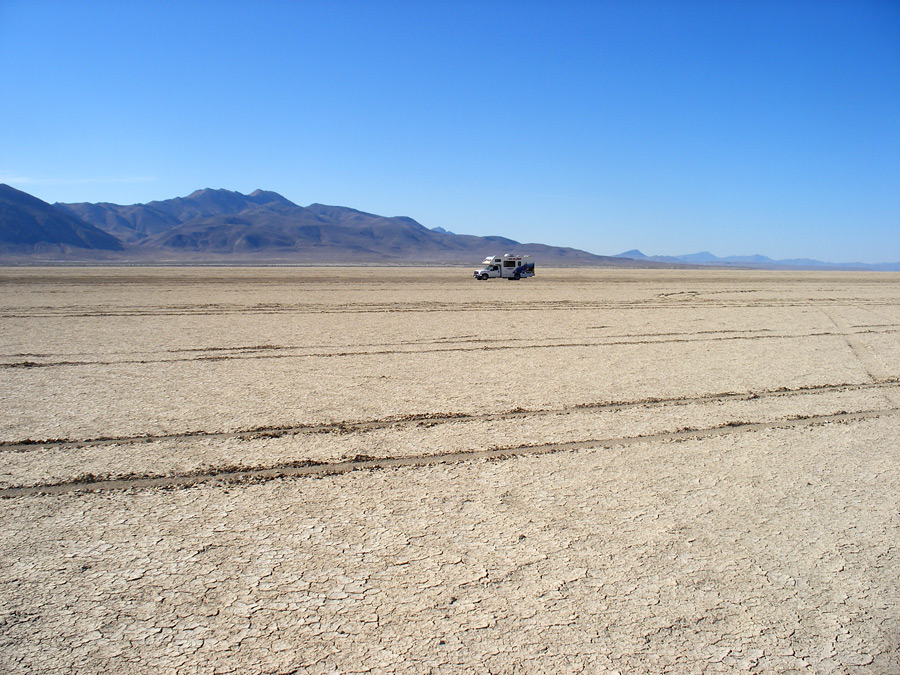
\includegraphics[width=0.6\textwidth]{blackrock}
    	\caption{Original image of Black Rock Desert, Nevada.}
	\vspace{1.5cm}

	\centering
	\captionsetup{justification=raggedleft, margin=3.6cm,singlelinecheck=off}
	\hfill
    	
\includegraphics[width=0.6\textwidth]{thresh}
    	\caption{Sample image utilizing a threshing filter.}

\end{figure}
\newpage
\begin{figure}
	\captionsetup{justification=raggedright, singlelinecheck=off}
    	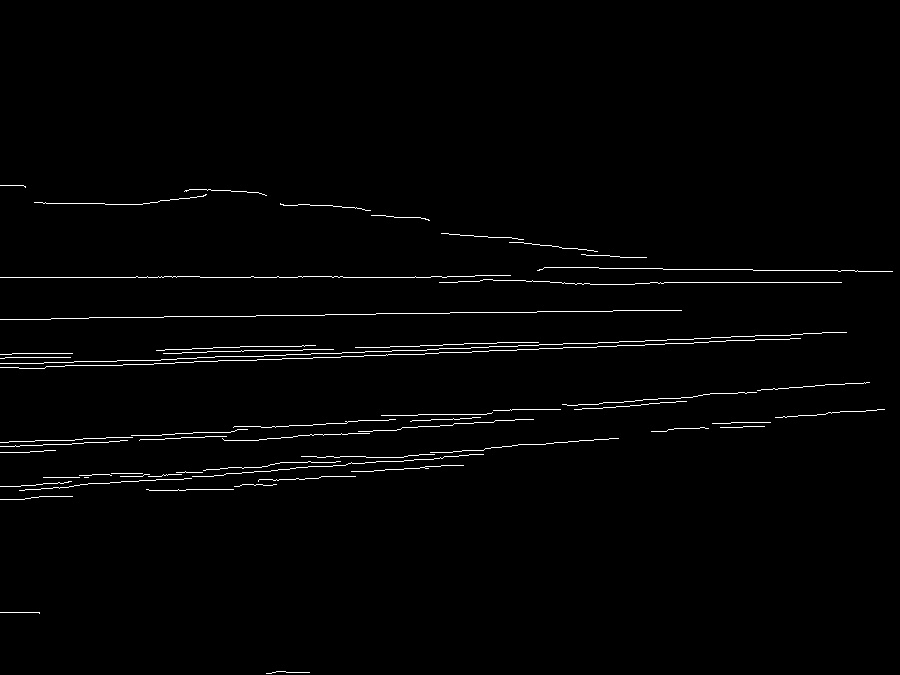
\includegraphics[width=0.6\textwidth]{canny}
    	\caption{Sample image utilizing a Canny filter.}

\end{figure}

\subsubsection{Week 4}\hspace*{\fill}\\
In the fourth week our team met with our mentor, as well as, our client. The client showed up at our team meeting which proved to be very beneficial. We were able to get many of our questions answered or directed to the appropriate resource to get the questions answered. There were also important decisions made at the meeting regarding the hardware we will be working with. Since this team meeting we have officially known all the hardware which we will be interacting with! This was one of the weeks where we had a lecture for capstone. At this lecture we were given an assignment description of the midterm progress report. The alpha version prototype requirements were defined in this lecture by Dr. McGrath as well. His description of the alpha prototype made it seem far more realistic to complete by week 6 which helped relieve much of my stress.\vspace{.3cm}
\par
As far as progress on the project, In week 4 I was able to get in contact with Bill Smart who is one of the leading researchers in robotics and machine learning here at OSU. He put me in contact with some of his grad student researchers so that I could get some assistance working on the object detection algorithm. By the end of this week, I had still not heard back from them, but merely gaining his assistance is a huge step in learning how to implement the object recognition that will be used in the final stage of the satellite's trek.\vspace{.3cm}
\par
\subsubsection{Week 5}\hspace*{\fill}\\
In week 5, our team met with the other engineers working on our project and with our client again on Tuesday. We had a lecture this week as well, and some new assignments were discussed. One of the assignments was the progress report. Our team was assigned to update the original progress report document with each of our progress over the last five weeks. We were also informed that we needed to record another presentation for our project which should be approximately 30 minutes long. We were also informed that we needed to update all documents from the previous term if any of the information in them had changed. After making the necessary changes, we were instructed to publish them in a OneNote notebook.\vspace{.3cm}
\par  
In this week, I created the OneNote notebook for our project and I've been working with some of Bill Smart's graduate students to develop a machine learning algorithm for locating the pole at the end of our satellite's trek. These types of algorithms are pretty foreign to me, and we still do not know exactly what the target will look like, so there was not and will not be a way that it gets finished before the alpha release but hopefully for our beta release. I've been conducting a lot of research on machine learning object recognition and it is extraordinarily interesting to me. This may be the most interesting chunk of code I will have developed by the time it's finished.\vspace{.3cm}

\subsection{Steven Silvers}
This section details the progress made by team member Steven Silvers during the first half of winter term  as well as any work done over winter break. Steven is responsible for making sure the control board for our project will provide what we need, and for determining what kind of wheel system our rover will use. The biggest piece that Steven is responsible for is the obstacle avoidance module, which is the main tool used by our autonomous driving system to keep our rover from becoming stuck during the competition.

\subsection{Week 1}
Start of winter term, over break I studied various autonomous driving methods since that is the main part of the project I am responsible for. I also looked at different hardware implementations and how they would possibly effect our programming decisions. We are communicating with the rest of the ARLISS capstone team to find a weekly meeting time, and have set our weekly TA meeting for Tuesdays at 1:30pm. Hopefully our whole team meeting time will be set soon so the ECE and ME teams can update us on their progress.

\subsection{Week 2}
Week two we met with our TA Franks for the first time this term, and discussed what is expected of the group as far as implementation of our project for this term. We as a group decided what a successful alpha version of our project would look like. We decided since the other two teams on our project would mostly likely not be finished with the hardware implementation until the end of the term, that for our alpha release we would write simulators for our individual modules to demonstrate that they function properly. The goal for the Beta release is to have the code implemented on hardware, but that is entirely dependent on the progress made by the ME and ECE groups.


\subsection{Week 3}
Week three we held a team wide meeting with the ECE and ME groups to better figure out time lines and what everyone is working on. It sounds like the ECE team has finally settled on using a Raspberry Pi zero as the main board for the rover, giving us a better idea of how we need to implement our code. The ME team told us that they will be designing and creating the wheel system in house so that it is fully customized to meet our needs. Progress has continued to be made on developing and simulating our individual code pieces in preparation for the week 6 alpha release.

\subsection{Week 4}
This week was mostly business as usual, we continued working on the alpha version of our project, as well as had an all group meeting that included our client Dr. Squires. My development module has been changed in that it will be getting a .mat file as input instead of a 2d binary array. This change will need to be reflected in the requirements document. As it is a late change, the alpha version will still be making use of a 2D binary array, and the plan is to change over to the .mat file for the beta version.

\subsection{Week 5}
Week five was spent doing work on the alpha version of the modules I am responsible for, mostly the obstacle avoidance system. Because of this modules' complexity it was decided that the alpha would be a lower level "prof of concept" and full functionality would be added by the 1.0 release. I edited both the tech review and the design document to reflect changes that had been made to the project for the sections I am responsible for. The biggest edit was for the control board, reflecting the decision made by the ECE team to use a Raspberry Pi Zero instead of one of the previously listed options.

\subsection{Week 6}
Week six was focused entirely on the upcoming alpha release and progress report. We decided that each team member would write their pieces individually and then combine them into one document Thursday, giving us plenty of time to submit the report on Friday. We got together with the ECE and ME teams for our weekly meeting, which ended early because all three groups were busy with progress reports and had nothing of significance to share. The ME team is uncertain of their capstone number, which hopefully they will figure out soon so that we can register as a group for Expo. The ME team also revealed to us during the short meeting that the rover frame did not hold up in testing and broke. They are now considering manufacturing the frame to the rover out of acrylic as it is a sturdy lightweight material that they believe will be easier to work with.

\subsection{Control Board}
Progress for the control board module so far consists of coming together with the ECE and ME teams and selecting what board we would like to use for the project. At our first all group meeting we decided that a Raspberry Pi Zero would be the best fit for our project given the size constraints and the processing power needed by our imaging system. Once that decision was made, it was a matter of placing the order for the Pi Zero boards and updating the technology review and the design document to reflect the decision to use the Pi Zero.
\begin{figure}[h!]
	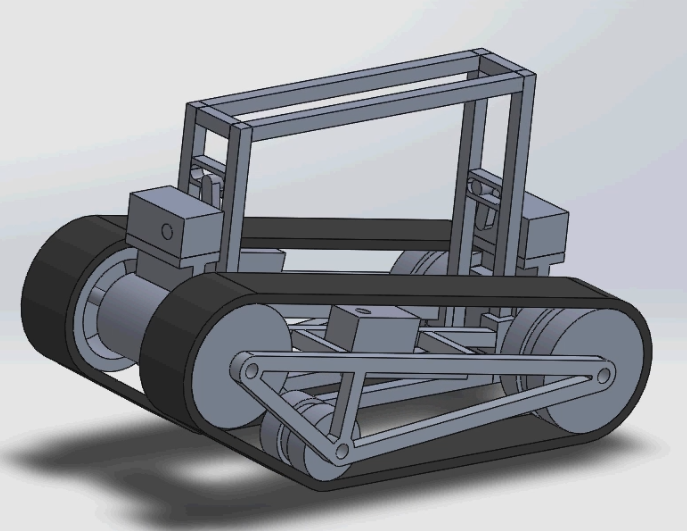
\includegraphics[scale = .4]{Capture.PNG}
	\caption{SolidWorks design of the rover}
	\label{fig:rover}
\end{figure}
\subsection{Wheel System}
The wheel system for our rover will be designed and manufactured by our project's ME team here at Oregon State. As shown in figure \ref{fig:rover}, our wheel system is a caterpillar track featuring three wheels per track, one of which is connected to a motor while the other two are for stabilization and guidance. Currently only the design for the wheel system has been created, the wheel system should be produced and ready for testing by the beta release.


\subsection{Obstacle Avoidance}
The obstacle avoidance system is what took up most of my time so far this term, as it is proving to be one of the trickier modules. I spent part of winter break as well as the first few weeks of winter term just focused on research for how to best implement a solution to this problem. The current plan is to take in a 2D binary array as input where ones represent edges detected in an image, and zeros are unchanging terrain.
\begin{figure}[h]
	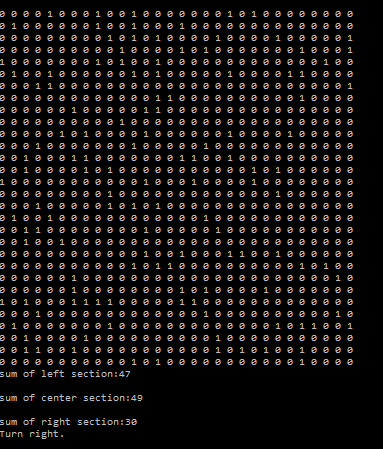
\includegraphics[scale = .75]{obstacleavoidance.png}
	\caption{current output from alpha version}
	\label{fig:obstacle}
\end{figure}
\par
The obstacle avoidance algorithm splits the array into three large columns, left, center and right, and then sums those columns. This summation tells us where the most edges are, which translates to where the roughest terrain is. In figure \ref{fig:obstacle} it shows that the sum of the right column was the lowest, so the rover should turn right to avoid the rougher terrain in front of it and to the left. For testing purposes, the array used in the alpha release is randomly populated with ones and zeros. The current plan is for the beta version to be tested with actual images to ensure accuracy and logical correctness of the algorithm.

\subsection{Zhaolong Wu}
This section contains the Zhaolong's progress throughout the first 6 weeks of winter term. In the Arliss CanSat project, computer science sub-team, Zhaolong is responsible for the CanSat's navigation system design, payload fairing protocol development, and getting CanSat unstuck if its fell sideways. Though the most important part is the navigation system design, which is Zhaolong's main focus during this 6 weeks of research and development period.

\subsection{Week 1}
During the first week of the winter term, the team had one class meeting and instructor McGrath officially announced that we are in the implementation phase of the capstone project, the team setup the mentor meeting time on every Tuesday 11:30pm to fit every team member's schedule. The team is still waiting on the new weekly team meeting time with the ECE and ME team, and we are going to talk with the client to let her come to the first team meeting to give us a general direction. 

During the winter break I spent handful amount of time on researching the autonomous driving vehicle \&robot, especially on how navigation system is implemented on them, hopefully we can get our first prototype done soon.

\subsection{Week 2}
In winter term week 2, we met our TA for the first time this term. We set the weekly meeting with him on Tuesday 1:45-2:00 pm, he mentioned during the meeting of that week that the basic structure of this term in terms of our project, we have two major checkoffs, alpha version which will happen in midterm and beta version that I believe would be the final. So we suppose to have a functional prototype done by the midterm despite this is way beyond of our control because we have to get the ME team and ECE team to finish the actual rover then we can start to program it. So we have settled down that we will have something simulations done by the midterm, and each person in the group will be in charge with topics that we wrote in the tech-review from last term. We will have to send an email to the TA to specify though.
Other than that, we didn't have to much, I'm still doing researches on my part which I believe that's what every team member is doing at this moment, we still have not met, or heard any people in the ECE and ME team yet, we hope we will do next week.

\subsection{Week 3}
During the week 3 we finally had the first all major groups together meeting this week, we set the weekly meeting time on Tuesday from 6-7pm. The meeting went very well and it was surely very informative for our computer science sub-team, the mechanical team told us the specs of the rover design and what there schedule looks like for the winter term, just like us, they also need to have a working version of prototype to be done by the week 6, the working version means the rover has to be ready to be tested, under basic functional requirements. For example, being able to drive from given waypoint A to B, driving around a circle, etc.

We split work for now to the alpha version release, Zach is going to continuing working on the camera, Zhaolong is going to work on how to use GPS data, Paul is going to work on the parachute deployment and Steven is going to deal with the board.

\subsection{Week 4}
During the week 4 of winter term the team had 2 major parts done, during the all group weekly meeting, the ME team leader Kyle laid out the projected expense, as well as how much for now to make one single rover, which is roughly about 299 dollars. As the CS team for now we just need 2 Pi Zeros and one camera. Our client Dr.Squires showed up as well. We discussed some details of the CanSat competition, like what the target pole looks like in order to program the vision system. Per competition rule the rover need to have the GPS coordinates recorded in a time interval, which is fairly easy task, we are planing to put a little script in our program that let it create a log file automatically at the end.

During Thursday's class meeting, both instructors went through things we need to do in the future of the term, I'm aware that first we need a team leader, due to the over crowded classroom and the time conflicts with another class, I wasn't able to find the team members and had to leave class early, I will send out an email to ask.

\subsection{Week 5}
During week 5, we were mainly focus on revising the design document and get the mid-term assessment ready. I'm still trying to test the gps functions like feed dummy data in and trying to see the systems response. Also I did some researches only and wrote a obstacle detection pseudo code. Next week we will finish up our progress report and get more testing done. 
\begin{figure}[h]
	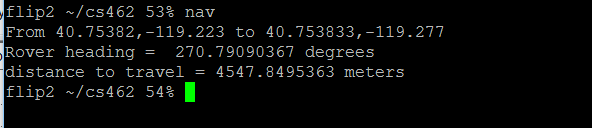
\includegraphics{navout.png}
	\caption{Current output from navigation system.}
	\label{fig:Navigation}
\end{figure}
\begin{figure}[h]
	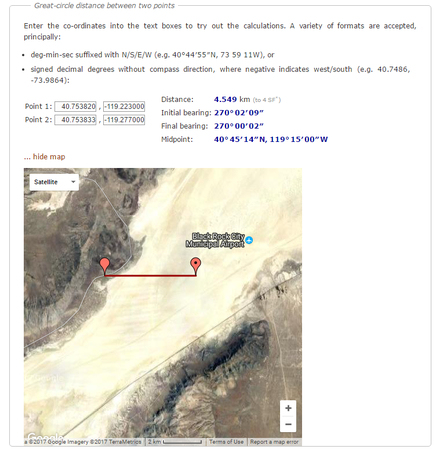
\includegraphics{testout.png}
	\caption{Comparing current output from navigation system with online GIS source.}
	\label{fig:Navigation1}
\end{figure}
\newpage

\subsection{Week 6}
During week 6, I spent most of the time to do more testing on the navigation system, the two output images above shows that the algorithm in the navigation program for getting the shortest path and initial heading, the output is matching the online GIS calculator. I'm currently waiting on to get the GPS, pcb board, and motor controller, etc. from the ECE team so I can do the integration tests. For the current testing method I used the location coordinates from the competition site Black Rock, NV, I hard coded two sets of coordinates as start point and finish pole.  


\subsection{Future of the term}
For the second half of the term, I will have to do more integrate tests, to ensure that the navigation system will working, as well as the payload fairing protocol and mechanical arm control. The system integration will be our goal for the beta version, so we can have a fully functional platform that allows us to perform further complex tests on.
\par

\subsection{Paul Minner}
Paul Minner is responsible for three modules on this project. They are for parachute deployment, getting unstuck from obstacles, and finding/touching the finish pole. Parachute deployment is fairly simple, we just deploy the parachute once below a certain altitude. Getting unstuck from obstacles is more difficult. Since we don’t yet have access to the rover itself, I had to make assumptions about what would work. Currently, I am attempting to back up the rover, and then rotating it if I don’t detect that the rover has moved, and backing up again. This module may change significantly once we have access to the rover and we can test it. Finally, finding/touching the finish pole is also difficult. Once the rover navigates to within the GPS error range of the finish destination, we have to switch to this mode. There is a pole that the rover needs to hit, so we use the camera to search for the pole so we can drive into it. Another team member is in charge of detecting the pole in the image, but I am in charge of using that data to direct the rover to hit the pole itself. At the beginning of this term, I had determined how I was going to implement these modules, but I hadn’t written any code yet. Here is a week by week summary of my progress over this term. 
\subsection{Week 1}
This week, we started getting back into the swing of things. We've scheduled our weekly meetings with our TA for 11:30 AM Tuesday, and are currently getting our weekly meetings with the entire group figured out. Over break I researched about the components needed for the parts of the project I'm responsible for, such as GPS and cameras. I learned that the GPS error for altitude is actually about 1.5 times worse than horizontal coordinate error, which is good to know for the parachute deployment module. Soon, I should begin actually implementing my design. Our only implementation problem is that the hardware isn't available yet, and therefore we will have to simulate it. In my case, that means simulating the GPS altitude, and the camera with obstacle detection.
\subsection{Week 2}
This week, we didn't accomplish much. Mostly, we started planning what parts need to be completed for the alpha build due during week 6 of the term. For me, that means I need a working simulation of each of my modules by week 6. This was a challenge, because my module to find and touch the finish pole relies on another teammate’s task to detect the finish pole itself. I had to think of a way to simulate his part of the task for now. The entire ARLISS team is working on setting up a time for group meetings. Currently, Wednesdays at 6pm - 7pm is thought to be the time.
\subsection{Week 3}
This week, we finally met with the entire ARLISS group. At the meeting, we discussed where each group was, and upcoming due dates. We also finally know exactly what hardware we will be implementing our software on, which is a Raspberry Pi Zero. Each member of our group has been working on implementing their portions of the project, and will continue to do so next week. I have made significant progress on the parachute deployment module, and started working on the getting unstuck from obstacles module. There should also be another large group meeting next Tuesday to discuss progress with the other teams. Simulating hardware components for our modules has still been a challenge. Some components are difficult to simulate, which means we won't know exactly how the software will react until the hardware is finished and we can test the rover itself. Other than that, simulating most modules of our software for the alpha build seems doable.
\subsection{Week 4}
This week, we continued to work on the alpha release of our project. We also got our OneNote page set up. We are beginning to revise our documents to reflect recent changes in our plans, and we need to write our progress report. My technology pick for finding and touching the finish pole on the tech review turned out to not actually be what we used, so I changed that, as well as made minor changes to the algorithms I use on the design document for the separate modules. 
\subsection{Week 5}
This week, we made significant progress on our modules in preparation for the upcoming progress report and demo. I finished the Parachute Deployment Module, as well as the Getting Unstuck From Obstacles module, with testing programs for each module. I ended up simulating the GPS by decreasing the altitude value by a fixed amount every time the altitude function was called, and I simulated finding the finish pole by returning a true value randomly 1/6 of the time. These simulations just ensure the algorithms will work correctly under currently anticipated conditions. We will have to test the entire program with the hardware to discover edge cases we didn’t anticipate, but that will be done later.
\subsection{Week 6}
We’ve finally made it to our current progress. This week, I finished up the find and touch the finish pole module, so all programming I need to complete for the alpha release is done. I have also worked on writing this progress report, and am currently working on the presentation. Everything is going smoothly, and we should have no problem hitting the friday deadline for the alpha release.
\subsection{Future}
In summary, I managed to create a working testing programs for each of my modules. All data from the sensors are currently simulated, so it’s still difficult to know how well my modules will work in the real world. I do know, however, that they will at least work for anticipated conditions, and there are no logical errors with them.
\begin{figure}[h]
  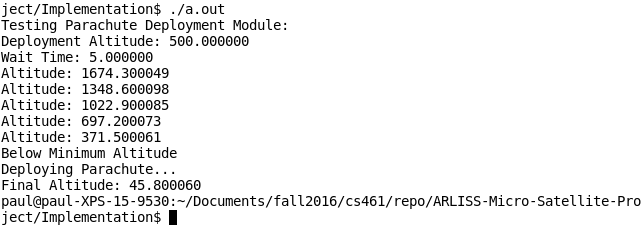
\includegraphics{parachuteoutput.png}
  \caption{Current output from parachute deployment simulation.}
  \label{fig:parachute}
\end{figure}
\par
Over the rest of this term, I will need to integrate my modules with the rest of the team’s pieces to create one large program. Once we have a single program, we can create better tests to better simulate the system as a whole. This should be our goal for the beta release at the end of this term. By then, the engineering teams should be finished up with the hardware components, so next term we can test the hardware itself. That means next term, we will focus on testing our software in the real world, and making any changes to ensure the rover succeeds at the competition. 

%\section{References}

%\bibliographystyle{IEEEtran}
%\bibliography{tech}

\end{document}
